\chapter*{\textsc{Introduction}}
\addcontentsline{toc}{chapter}{\textsc{Introduction}}
	
	\paragraph{}
		Cette manipulation se propose de réaliser un asservissement de position en mettant en œuvre les techniques d’espace d’état continu. Le procédé utilisé est la platine ”asservissement de position" qui apparaît dans la \hyperref[fig1]{Figure 1}, déjà présentée dans les textes des manipulations des TP de licence EEA (2ème année) dont le principe est rappelé sur le schéma présenté dans la \hyperref[fig2]{Figure 2.}

	\begin{center}
	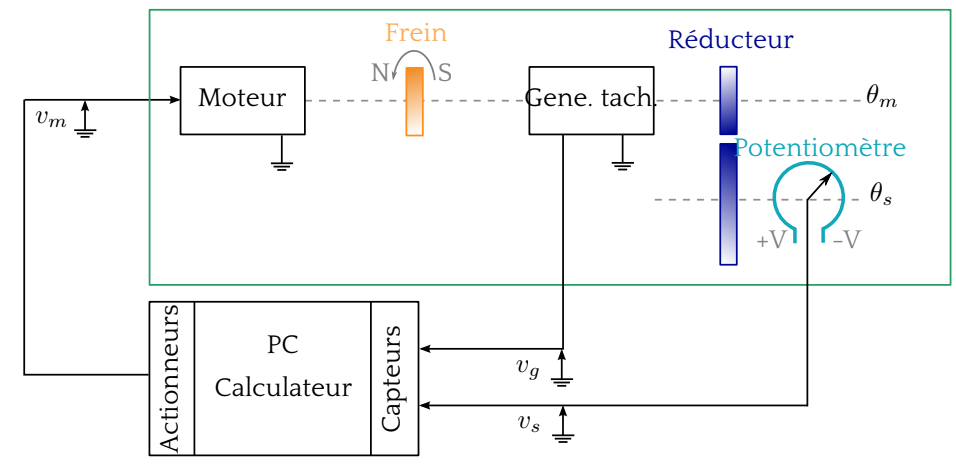
\includegraphics[scale=0.4]{schemamotor.png}
	\captionof{figure}{\textit{Asservissement de position par calculateur\\}}
	\label{fig1} 
	\end{center} 
	
	\begin{center}
	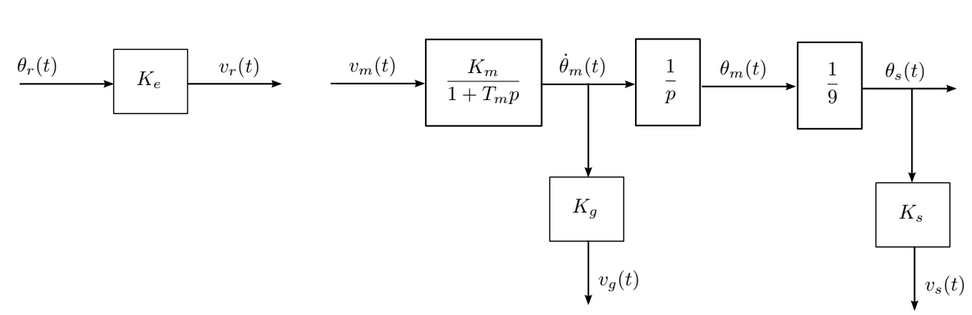
\includegraphics[scale=0.4]{schemablocmotor.png}
	\captionof{figure}{\textit{Eléments de la platine (asservissement de position)\\[4cm]}}
	\label{fig2} 
	\end{center}
	
	\begin{itemize} [label=\ding{70},font=\small \color{black}]
	\item $v_{m}(t)$\hspace{1mm} est la tension d'entrée du moteur.
	\item $\theta_{s}(t)$\hspace{1mm} est la position de l'axe secondaire du moteur.
	\item $\dot{\theta}_{m}(t)$ est la vitesse de rotation de l'axe principal du moteur.\\
	%Les paramètres $K_{m}$ et $\tau_{m}$ ont déjà été déterminés lors du TP2 de SLI1. 
	Les coefficients connus sont $K_{e}$, $K_{s}$ et $K_{g}$, leurs valeurs numériques sont données comme suit:
	\begin{itemize} [label=\ding{171},font=\small \color{black}]
	\item $K_{e} = 10(V.tr^{-1})$
	\item $K_{s} = 10(V.tr^{-1})$
	\item $K_{g} = 0.105(V.s.tr^{-1})$
	%\item $K_{m} = 10$
	%\item $K_{g} = 0.29(s)$
	\end{itemize}
	\end{itemize}
	
	\paragraph{}
		Il est possible d’obtenir une mesure de $\theta_{s}(t)$ et de $\theta_{m}(t)$ via un potentiomètre et une génératrice tachymétrique.
		
		\begin{center}
		$v_{m}(t) = K_{s}\theta_{s}(t)$ \hspace{1.5cm} et \hspace{1.5cm} $v_{g}(t) = K_{g}\dot{\theta}_{m}(t)$ 
		\end{center}
		
